\documentclass{article}

\usepackage{corl_2026}

\usepackage[utf8]{inputenc}
\usepackage[T1]{fontenc}
\usepackage{amsmath,amssymb,amsfonts}
\DeclareMathOperator*{\argmin}{arg\,min}
\DeclareMathOperator*{\argmax}{arg\,max}
\usepackage{graphicx}
\usepackage{booktabs}
\usepackage{enumitem}
\usepackage{multirow}
\usepackage{wrapfig}


\graphicspath{{figures/}}
\setlength{\textfloatsep}{6pt plus 1pt minus 1pt}
\setlength{\floatsep}{6pt plus 1pt minus 1pt}
\setlength{\intextsep}{6pt plus 1pt minus 1pt}
\setlength{\abovecaptionskip}{4pt}
\setlength{\belowcaptionskip}{-2pt}
\setlength{\abovedisplayskip}{6pt plus 2pt minus 2pt}
\setlength{\belowdisplayskip}{6pt plus 2pt minus 2pt}
\setlength{\abovedisplayshortskip}{2pt plus 1pt}
\setlength{\belowdisplayshortskip}{4pt plus 1pt minus 1pt}

\title{Knowing When Not to Correct:\\ Adaptive Test-Time Refinement for Vision-Language-Action Models}

\author{
  Anonymous
}

\begin{document}

\maketitle

\setlength{\parskip}{0pt plus 0.5pt}

\begin{abstract}
Learned post-hoc correction of frozen flow-matching Vision-Language-Action (VLA) models is harmful by default. The problem is not the correction module itself but its unconditional application: on most control steps the VLA already produces confident, low-variance actions, and corrections applied here act as noise---degrading all four LIBERO manipulation suites on SmolVLA (0.4B) by up to $-$14.8\,pp under a K-matched controlled comparison. We propose calibrated uncertainty gating: $K{=}2$ stochastic action samples are drawn in a single batched forward pass at zero extra latency (${\sim}$170\,ms, matching $K{=}1$), and their pairwise $L_2$ distance gates a lightweight (${\sim}$327K parameter) correction module so that only genuinely uncertain steps receive learned residual correction. Selective gating recovers up to $+$13.5\,pp of the degradation caused by unconditional correction, restoring near-baseline or above-baseline performance across all four suites. The trigger rate (fraction of corrected steps) shows a positive trend with net improvement over VLA-only, providing a built-in deployment diagnostic. Experiments on $\pi_{0.5}$ (3.6B) with $n{=}3$ seeds per condition confirm that the degradation pattern persists and amplifies ($-$17.5\,pp on Long), with partial recovery from gating. The key finding is that knowing when \emph{not} to correct matters more than the correction itself.

\end{abstract}

\keywords{Vision-Language-Action Models, Inference-Time Refinement, Robotic Manipulation}

\section{Introduction}
\label{sec:intro}

Frozen flow-matching Vision-Language-Action (VLA) models offer a compelling deployment paradigm: a single pretrained policy can handle diverse manipulation tasks without retraining~\cite{black2024pi0,shukor2025smolvla,lipman2023flow}. Yet their action quality is bounded by the pretrained weights, and fine-tuning remains expensive when new tasks arrive frequently. Post-hoc learned correction, a lightweight module that refines actions at inference time without modifying VLA weights~\cite{snell2024scaling}, is an appealing alternative. But does it actually help?

\begin{figure}[t]
  \centering
  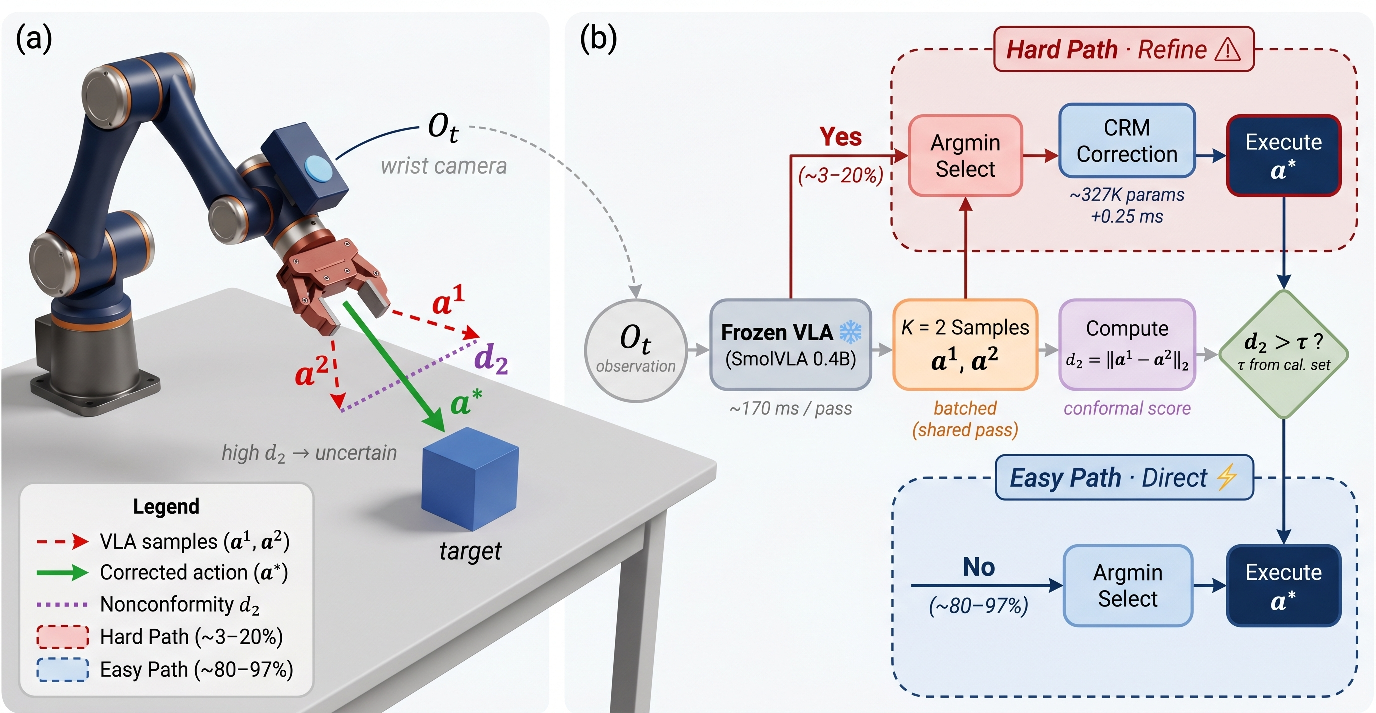
\includegraphics[width=\linewidth, trim=2 0 7 11, clip]{fig1_pipeline.pdf}
  \caption{Calibrated gating pipeline. $K{=}2$ action samples are drawn from the frozen VLA; their pairwise $L_2$ distance forms a calibrated uncertainty score. When the score falls below $\tau$ (confident step), the argmin-to-centroid sample is output directly. When it exceeds $\tau$ (uncertain step), a lightweight Correction Residual Module (CRM) applies bounded correction ($\|\boldsymbol{\delta}\|_2 \leq \varepsilon$).}
  \label{fig:pipeline}
\end{figure}

We systematically evaluate this idea and find a surprising negative result: unconditional learned correction is consistently harmful across all evaluated configurations. Across four LIBERO manipulation suites~\cite{liu2023libero} and two VLAs spanning nearly an order of magnitude in scale (0.4B to 3.6B), applying a correction module at every control step consistently degrades performance (Section~\ref{sec:failure_modes}). The problem is not the correction module itself, but the assumption that every step needs correction.

Prior work either corrects unconditionally~\cite{a2c2_2025}, quantifies uncertainty without learned correction~\cite{chen2026reconvla}, or requires RL~\cite{liu2026scvla} or slow evolutionary search ($2.41$\,s/step)~\cite{li2025vlapilot}. None analyze when correction helps versus hurts, nor provide a mechanism to suppress it on confident steps.

Our analysis reveals the root cause: on the four evaluated suites, 80--97\% of control steps already produce confident, near-deterministic actions; corrections on these steps inject noise rather than signal. The direct consequence is that knowing \emph{when not to correct} matters more than the correction's magnitude---the correction module is effective, but only on the 3--20\% of steps where the VLA is genuinely uncertain. We propose a simple gating mechanism: two stochastic action samples drawn in a single batched forward pass provide a per-step uncertainty estimate at zero extra latency. A calibrated threshold on their pairwise distance gates correction to the small fraction of genuinely uncertain steps, while the VLA's own output passes through on confident steps. This selective prediction approach~\cite{chow1970optimum,geifman2017selective} restricts correction to the minority of steps where it is most needed.

On SmolVLA~\cite{shukor2025smolvla} (0.4B) across four LIBERO suites, selective gating recovers nearly all degradation from unconditional correction. Cross-VLA experiments on $\pi_{0.5}$~\cite{black2025pi05} (3.6B) with $n{=}3$ seeds per condition confirm that the failure pattern persists and amplifies on stronger models. Threshold sensitivity analysis shows that gating is robust to $\tau$ choice, and trigger rate shows a positive trend with net improvement over VLA-only across suites (Appendix~\ref{sec:tau_sweep}).

Our contributions are:
\begin{enumerate}[leftmargin=*,nosep]
  \item \textbf{Failure analysis of unconditional correction} (Section~\ref{sec:failure_modes}): we show that applying learned correction at every step degrades frozen VLAs across all evaluated task suites and model scales, and identify confident steps (where the VLA needs no help) as the source of harm.
  \item \textbf{Calibrated gating via pairwise uncertainty} (Section~\ref{sec:method}): two action samples yield a per-step uncertainty proxy that gates correction to the small fraction of uncertain steps, recovering nearly all degradation on SmolVLA at zero extra latency.
  \item \textbf{Cross-VLA validation and deployment guidelines} (Section~\ref{sec:experiments}; Appendix~\ref{sec:cross_vla}): the degradation pattern generalizes from SmolVLA (0.4B) to $\pi_{0.5}$ (3.6B) with $n{=}3$ seeds per condition, and five data-grounded deployment rules---including trigger rate as a zero-cost diagnostic---enable practitioners to predict whether correction will help for a given task distribution without full evaluation.
\end{enumerate}

\section{Related Work}\label{sec:related_work}

\paragraph{VLA robustness.} VLAs have progressed from tokenized prediction~\cite{brohan2023rt2,kim2024openvla,ghosh2024octo} to flow matching~\cite{black2024pi0,shukor2025smolvla}, yet lose over 65\,pp under deployment perturbations~\cite{fei2025liberoplus}. Training-time defenses~\cite{srpo2025,robustvla2025,digflow2025} and test-time RL adaptation~\cite{liu2026ttvla} improve robustness but require modifying VLA weights.

\paragraph{Inference-time correction.} Among frozen-VLA methods, ReconVLA~\cite{chen2026reconvla} quantifies uncertainty without learned correction; SC-VLA~\cite{liu2026scvla} trains auxiliary world-model heads for online refinement via reward reshaping; VLA-Pilot~\cite{li2025vlapilot} uses evolutionary search at 2.41\,s per step. Tang et al.~\cite{tang2026shifting} propose uncertainty quantification for VLAs via max-pooled sliding windows but do not learn corrective actions. A2C2~\cite{a2c2_2025}, the closest concurrent work, learns a correction head for temporal staleness but applies it unconditionally. Our pipeline detects \emph{when correction would hurt}, using calibrated gating to suppress correction on confident steps. Residual policy learning~\cite{silver2018residual,johannink2019residual} shares the additive structure; magnitude control is addressed by gating~\cite{jiang2024transic}, clipping~\cite{xiao2026pld}, or decay~\cite{pan2025drc}. Our CRM uses fixed $L_2$ clipping with supervised loss, requiring no RL.

\paragraph{Selective prediction.} Our $\tau$-gating is an instance of selective prediction~\cite{chow1970optimum,elyaniv2010selective,geifman2017selective}. Unlike SelectiveNet~\cite{geifman2019selectivenet}, we use a pairwise distance threshold with no additional learned components. The $K{=}2$ $L_2$ distance is a minimal ensemble disagreement measure~\cite{lakshminarayanan2017simple}, exploiting the inherent stochasticity of flow-matching generation rather than injected noise as in MC Dropout~\cite{gal2016dropout}, and requiring no architectural changes. Conformal prediction~\cite{angelopoulos2023gentle} has been applied to robotics~\cite{lindemann2023safe,zhao2024conformalized,yao2025cpnav}; our threshold draws on this calibration philosophy without formal coverage guarantees.

\paragraph{Inference-time scaling.} Test-time scaling in LLMs~\cite{snell2024scaling} uses best-of-N selection; RoVer~\cite{dai2025rover} and DA-SIP~\cite{chun2025dasip} extend this to VLAs. Our analysis reveals a different pattern: learned correction is harmful when unconditional, and the key mechanism is calibrated gating rather than scaling sample count (Section~\ref{sec:main_results}). To our knowledge, no prior work systematically examines \emph{when} post-hoc correction of frozen VLAs degrades performance or provides a calibrated mechanism to selectively suppress it. We address both the analysis---establishing that unconditional correction is universally harmful across tasks and model scales---and the method: adaptive gating that makes learned correction safe to deploy.


\section{Method: When to Apply Learned Correction}
\label{sec:method}

\begin{figure}[t]
  \centering
  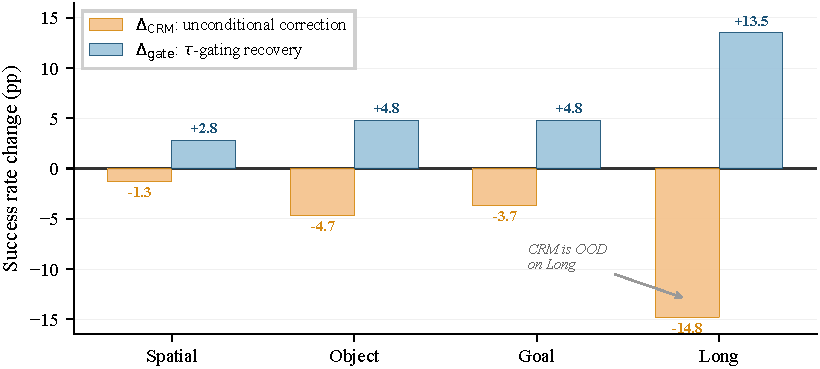
\includegraphics[width=\linewidth]{fig_teaser.pdf}
  \caption{Degradation from unconditional correction ($\Delta_{\mathrm{CRM}}$, orange) vs.\ recovery from calibrated $\tau$-gating ($\Delta_{\mathrm{gate}}$, blue) across four LIBERO suites on SmolVLA. Unconditional CRM correction degrades all suites (up to $-$14.8\,pp on Long, where the CRM is out-of-distribution); $\tau$-gating recovers nearly all degradation by restricting correction to high-uncertainty steps.}
  \label{fig:teaser}
\end{figure}

We propose a calibrated gating pipeline for frozen flow-matching VLAs (Figure~\ref{fig:pipeline}). The calibration is based on held-out percentile thresholds of pairwise distances; it does not implement formal conformal prediction guarantees~\cite{angelopoulos2023gentle}. Since unconditional learned correction degrades all evaluated suites (Section~\ref{sec:failure_modes}), the pipeline uses a $K{=}2$ pairwise distance to decide per step whether correction is safe. At each control step, the pairwise $L_2$ distance between two stochastic action samples forms an uncertainty score; confident steps output the selected sample directly, while uncertain steps apply a learned residual correction via a lightweight Correction Residual Module (CRM). The base VLA is never retrained.

\subsection{Problem Setup}
\label{sec:problem_setup}

Let $\pi_\theta$ be a frozen flow-matching VLA that, given an observation $o_t$ (image, language instruction, proprioceptive state), generates action chunks of length $C{=}50$ in $\mathbb{R}^{d \times C}$ with $d{=}6$ (3 translation + 3 rotation). Under receding-horizon execution, only the first $H{=}5$ steps of each chunk influence the robot before re-planning, so we discard the remainder. The gripper dimension is handled separately via direct thresholding and is excluded from the pipeline.

Each forward pass of $\pi_\theta$ produces a stochastic action sample; querying independently $K$ times yields $K$ candidate chunks. Our goal is to produce a single action more accurate than any individual sample, with no changes to $\pi_\theta$. The method applies to any stochastic generative policy---including diffusion policies~\cite{chi2023diffusion_policy} and flow-matching VLAs---that produces diverse action samples (Appendix~\ref{sec:applicability}).

\subsection{Multi-Sample Selection}
\label{sec:selection}

We draw $K$ action chunks from $\pi_\theta$ via independent flow-matching rollouts and truncate each to $H{=}5$ steps, yielding samples $\{a_h^{(k)}\}_{k=1}^K$ with $a_h^{(k)} \in \mathbb{R}^d$ for horizon step $h = 1, \dots, H$. For each step, we compute the sample mean $\boldsymbol{\mu}_h = \frac{1}{K}\sum_{k=1}^K a_h^{(k)}$ and select the sample with the smallest total $L_2$ distance to the mean across all horizon steps:
\begin{equation}
  a_{\mathrm{base}} = \argmin_{k \in \{1,\dots,K\}} \sum_{h=1}^{H} \bigl\|a_h^{(k)} - \boldsymbol{\mu}_h\bigr\|_2^2.
  \label{eq:argmin}
\end{equation}
Unlike the element-wise mean, which can blend incompatible modes, the argmin returns an actual sample and preserves within-sample temporal coherence. At $K{=}2$, the argmin-to-centroid cost is identical for both samples ($\|a^{(1)} - \boldsymbol{\mu}\| = \|a^{(2)} - \boldsymbol{\mu}\| = \|a^{(1)} - a^{(2)}\|/2$), so selection reduces to a deterministic index tie-break; the value of $K{=}2$ lies not in selection quality but in the pairwise distance signal for gating (Section~\ref{sec:adaptive_k_method}).

\subsection{Correction Module (CRM)}
\label{sec:crm}

The CRM is a lightweight MLP that refines the selected action $a_{\mathrm{base}}$ by predicting a bounded residual correction conditioned on the current observation and the selected action itself.

\paragraph{Architecture.}
The CRM consists of three fully connected layers with ReLU activations: $\mathrm{Linear}(n_{\mathrm{in}}, 256) \to \mathrm{ReLU} \to \mathrm{Linear}(256, 256) \to \mathrm{ReLU} \to \mathrm{Linear}(256, H{\cdot}d)$, preceded by input normalization. The input is the concatenation of the frozen observation embedding $\mathbf{z}_{\mathrm{obs}} \in \mathbb{R}^{n_{\mathrm{obs}}}$ from the VLA's vision-language encoder and the selected action $a_{\mathrm{base}} \in \mathbb{R}^{H \cdot d}$ ($H{=}5$ steps $\times$ $d{=}6$ degrees of freedom), giving $n_{\mathrm{in}} = n_{\mathrm{obs}} + 30$. The architecture is identical across VLAs; only $n_{\mathrm{obs}}$ differs ($960$ for SmolVLA, $2048$ for $\pi_{0.5}$), yielding $327$K--$615$K parameters ($<\!1$\% of either backbone). The output is a residual $\boldsymbol{\delta} \in \mathbb{R}^{30}$, and the corrected action is:
\begin{equation}
  \mathbf{a}^* = a_{\mathrm{base}} + \mathrm{clip}\bigl(\boldsymbol{\delta},\; \|\boldsymbol{\delta}\|_2 \leq \varepsilon\bigr),
  \label{eq:crm}
\end{equation}
where $\varepsilon$ is a norm bound that limits the correction magnitude (Section~\ref{sec:magnitude}). The CRM never sees individual action candidates: it receives only the already-selected $a_{\mathrm{base}}$ and predicts a correction toward the expert action. We tested alternative conditioning inputs (per-DOF uncertainty features, scalar uncertainty); observation-only conditioning performs best and is the primary variant.

\paragraph{Training.}
The CRM is trained offline on demonstration trajectories from LIBERO~\cite{liu2023libero} with $L_2$ loss:
\begin{equation}
  \mathcal{L} = \bigl\|\mathbf{a}^* - \mathbf{a}_{\mathrm{expert}}\bigr\|_2^2,
  \label{eq:loss}
\end{equation}
where $\mathbf{a}_{\mathrm{expert}}$ is the demonstration action. For each VLA, we precompute training data from 10 demonstrations per task across the target LIBERO suites. At each demonstration step, we run $K{=}10$ forward passes through the frozen VLA, apply argmin selection~(\ref{eq:argmin}) to obtain $a_{\mathrm{base}}$, and train the CRM to predict the residual toward $\mathbf{a}_{\mathrm{expert}}$. Training uses Adam ($\mathrm{lr}{=}10^{-3}$), batch size 32, 50 epochs, with Gaussian noise augmentation on $a_{\mathrm{base}}$ (static perturbation, not interactive aggregation as in DAgger~\cite{ross2011dagger}) to improve generalization to the closed-loop state distribution. Note that the CRM is trained on $a_{\mathrm{base}}$ obtained via $K{=}10$ argmin (well-centered sample), whereas at deployment with $K{=}2$ the argmin is degenerate (Section~\ref{sec:selection}), creating a train--test distribution shift that may partially explain CRM underperformance.

\subsection{Magnitude Control}
\label{sec:magnitude}

The norm bound $\varepsilon$ in~(\ref{eq:crm}) is critical for stable closed-loop performance. Without clipping, the CRM's unconstrained output norm (${\approx}$1.42) causes compounding errors. Constraining $\varepsilon$ to $[0.05, 0.2]$ yields stable corrections (Appendix Figure~\ref{fig:tau_sweep}b). Both CRM always-on and CRM $\tau$-gated use $\varepsilon{=}0.2$; the K-matched design ensures the only difference is gating (Section~\ref{sec:failure_modes}).

\subsection{Calibrated Uncertainty Gating}
\label{sec:adaptive_k_method}

Experiments reveal that unconditional correction is consistently harmful across all evaluated configurations: CRM applied at every step degrades all four LIBERO suites (up to $-$14.8\,pp; Section~\ref{sec:failure_modes}). The 80--97\% of steps where the VLA is already confident receive corrections that are noise. The solution is a calibrated gating mechanism that detects confident steps and suppresses correction accordingly.

\paragraph{Why $K{=}2$.}
$K{=}2$ is the minimum sample size that admits a pairwise disagreement measure, and under batched inference the uncertainty signal is \emph{free}: $K{=}2$ latency (${\sim}$170\,ms) matches $K{=}1$ because both samples share the same prefix encoding and flow-matching denoising runs in parallel (Table~\ref{tab:efficiency}). Empirically, the $K{=}2$ $L_2$ distance ranks steps in nearly identical order to $K{=}10$ sample variance ($\rho{=}0.9979$; Table~\ref{tab:proxy_comparison}), establishing ordering consistency of the proxy; this measures relative uncertainty ranking, not predictive validity for action correctness. Step-level validity is established indirectly through the suite-level positive correlation between trigger rate and net improvement over VLA-only (Figure~\ref{fig:trigger_scatter}). Three alternative probes, including CRM correction magnitude ($K{=}1$ and $K{=}2$) and flow-matching velocity dispersion (FMVD), all fail ($\rho < 0.16$). Under the K-matched comparison ($K{=}2$ for both), calibrated $\tau$-gating exceeds unconditional correction on all four evaluated suites ($\Delta_{\mathrm{gate}}{=}{+}2.8$ to $+$13.5\,pp; Section~\ref{sec:main_results}).

\begin{table}[t]
\centering
\caption{Uncertainty proxy comparison. Spearman $\rho$ between candidate proxies and $K{=}10$ action variance (ground-truth uncertainty), evaluated on LIBERO-Object (27{,}626 steps). Only pairwise $L_2$ distance achieves meaningful correlation.}
\label{tab:proxy_comparison}
\small
\begin{tabular}{lcc}
\toprule
Proxy & Spearman $\rho$ & Extra VLA calls \\
\midrule
$K{=}2$ pairwise $L_2$ (ours) & $\mathbf{0.9979}$ & 1 \\
$K{=}1$ CRM correction magnitude & $0.152$ & 0 \\
$K{=}2$ CRM correction magnitude & $0.134$ & 1 \\
Flow velocity dispersion (FMVD) & $0.083$ & 0 \\
\bottomrule
\end{tabular}
\end{table}

\paragraph{Three-step gating pipeline.}
At each control step, the pipeline executes:
\begin{enumerate}[nosep,leftmargin=*]
  \item \textbf{Uncertainty probe.} Draw $K{=}2$ samples $a^{(1)}, a^{(2)}$ from $\pi_\theta$ in a single batched forward pass. Compute the pairwise distance $d_2 = \|a^{(1)} - a^{(2)}\|_2$ and select $\hat{a}$ via~(\ref{eq:argmin}); at $K{=}2$, both candidates have equal cost to the centroid, so a deterministic index is used.
  \item \textbf{Gating decision.} If $d_2 \leq \tau$ (low uncertainty), output $\hat{a}$ directly, requiring no further computation. If $d_2 > \tau$ (high uncertainty), pass $\hat{a}$ to the CRM for correction.
  \item \textbf{Learned correction.} For high-uncertainty steps only, the CRM predicts a bounded residual: $\hat{a}_{\mathrm{out}} = \hat{a} + \boldsymbol{\delta}$, where $\boldsymbol{\delta} = \mathrm{CRM}(o_t, \hat{a})$ and $\|\boldsymbol{\delta}\|_2 \leq \varepsilon$~(\ref{eq:crm}). The pipeline uses at most $K{=}2$ forward passes; performance gains come from learned correction, not brute-force sampling.
\end{enumerate}
The threshold $\tau$ is a percentile of the empirical $d_2$ distribution from CRM training data; it controls a precision--recall tradeoff: lower $\tau$ corrects more steps (higher recall, but risks correcting confident steps), while higher $\tau$ corrects fewer steps (higher precision, preserving baseline on confident steps). The optimal percentile is task-difficulty-dependent (Appendix~\ref{sec:tau_sweep}). CRM inference adds ${\sim}$0.25\,ms; the VLA forward pass (${\sim}$170\,ms batched) dominates latency.


\section{Experiments}
\label{sec:experiments}

We investigate when test-time correction helps or hurts on SmolVLA~\cite{shukor2025smolvla} (0.4B) across four LIBERO~\cite{liu2023libero} task suites. We ask: (i)~does unconditional correction degrade performance, and if so, why? (ii)~can calibrated gating recover the degradation? (iii)~what is the computational cost?

\begin{table}[t]
\centering
\caption{Task success rate (SR, \%\,$\uparrow$) on SmolVLA across four LIBERO suites. CRM always-on and CRM $\tau$-gated share identical $K{=}2$, $\varepsilon{=}0.2$, and CRM checkpoint; the only difference is whether correction is applied unconditionally ($\tau{\to}0$) or selectively (calibrated $\tau$). $\Delta_{\mathrm{CRM}}$: degradation from unconditional correction (CRM$-$VLA). $\Delta_{\mathrm{gate}}$: recovery from gating ($\tau$-gated$-$CRM). Trigger: fraction of steps where the calibrated gate fires.}
\label{tab:main}
\small
\begin{tabular}{lcccccc}
\toprule
Suite & VLA-only & CRM always-on & CRM $\tau$-gated & $\Delta_{\mathrm{CRM}}$ & $\Delta_{\mathrm{gate}}$ & Trigger \\
 & ($K{=}1$) & ($K{=}2$) & ($K{=}2$) & & & (\%) \\
\midrule
Spatial & $79.3 \pm 0.8$ & $78.0 \pm 1.7$ & $\mathbf{80.8 \pm 1.1}$ & $-1.3$ & $+2.8$ & ${\sim}20$ \\
Object & $77.7 \pm 1.3$ & $73.0 \pm 1.8$ & $\mathbf{77.8 \pm 3.0}$ & $-4.7$ & $+4.8$ & ${\sim}4$ \\
Goal & $83.7 \pm 1.3$ & $80.0 \pm 0.5$ & $\mathbf{84.8 \pm 1.5}$ & $-3.7$ & $+4.8$ & ${\sim}8$ \\
Long & $\mathbf{58.0 \pm 1.5}$ & $43.2 \pm 2.3$ & $56.7 \pm 2.3^\dagger$ & $-14.8$ & $+13.5$ & ${\sim}4$ \\
\bottomrule
\addlinespace[2pt]
\multicolumn{7}{l}{\scriptsize $n{=}3$ seeds unless noted. Bold: best per suite. $\tau$-gating recovers nearly all degradation; Long residual ($-$0.3\,pp) within noise.}\\
\multicolumn{7}{l}{\scriptsize $^\dagger$Long CRM $\tau$-gated: $n{=}5$ seeds (57.7\%); $n{=}3$ yields 56.7\%, difference within noise.}
\end{tabular}
\end{table}

\subsection{Setup}
\label{sec:exp_setup}

\paragraph{Benchmarks.}
We use all four LIBERO suites: Spatial (10 tasks, spatial reasoning), Object (10 tasks, novel object instances), Goal (10 tasks, goal specification), and Long (10 tasks, long-horizon manipulation). Each task is evaluated over 20 rollouts (max 300 steps, 200 per suite); success is binary.

\paragraph{Base VLA.}
SmolVLA~\cite{shukor2025smolvla} (0.4B parameters, flow matching) uses dual-camera RGB ($256{\times}256$), 8D proprioceptive state, and produces 7D actions (6D pose + 1D gripper, thresholded separately). We additionally report $\pi_{0.5}$~\cite{black2025pi05} (3.6B) baselines and OpenVLA-OFT~\cite{kim2024openvla} (7B) boundary analysis in Appendix~\ref{sec:cross_vla}.

\paragraph{Methods.}
All methods use the same frozen SmolVLA; no VLA weights are modified. \textbf{VLA-only} ($K{=}1$) uses a single forward pass with no correction. \textbf{CRM always-on} ($K{=}2$, $\varepsilon{=}0.2$, $\tau{\to}0$) applies argmin selection and CRM correction at every step; it shares the same $K$, $\varepsilon$, and CRM checkpoint as CRM $\tau$-gated, with calibrated gating disabled. \textbf{CRM $\tau$-gated} ($K{=}2$, $\varepsilon{=}0.2$, $\tau{=}0.25$) is the proposed calibrated gating pipeline (Section~\ref{sec:adaptive_k_method}), applying CRM correction only when $d_2 > \tau$.
Additional ablations ($K{=}10$ argmin~\cite{chen2026reconvla}, $K{=}2$ mean) are reported in Appendix~\ref{sec:additional_ablations}.

\paragraph{CRM training.}
The CRM (${\sim}$327K parameters) is trained on LIBERO demonstrations with 10 demos per task, $K{=}10$ forward passes each (Adam $\mathrm{lr}{=}10^{-3}$, batch 32, 50 epochs, $\varepsilon{=}0.2$). Both CRM always-on and CRM $\tau$-gated use the same CRM checkpoint and $\varepsilon$. The CRM is trained on three suites (Spatial, Object, Goal; 30 tasks, ${\sim}$88K samples). Long is \emph{not} included in CRM training; Long-suite evaluation therefore tests cross-suite generalization of the CRM (Appendix~\ref{sec:reproducibility}).

\paragraph{Statistics.}
We report mean $\pm$ std over $n$ seeds ($n{=}3$ unless noted). An extended 8-seed analysis on Spatial yields $p{=}0.017$ (Appendix~\ref{sec:8seed}). The primary comparison is CRM $\tau$-gated vs.\ CRM always-on under the K-matched design.

\subsection{Main Results}
\label{sec:main_results}
\label{sec:failure_modes}

\begin{figure}[t]
  \centering
  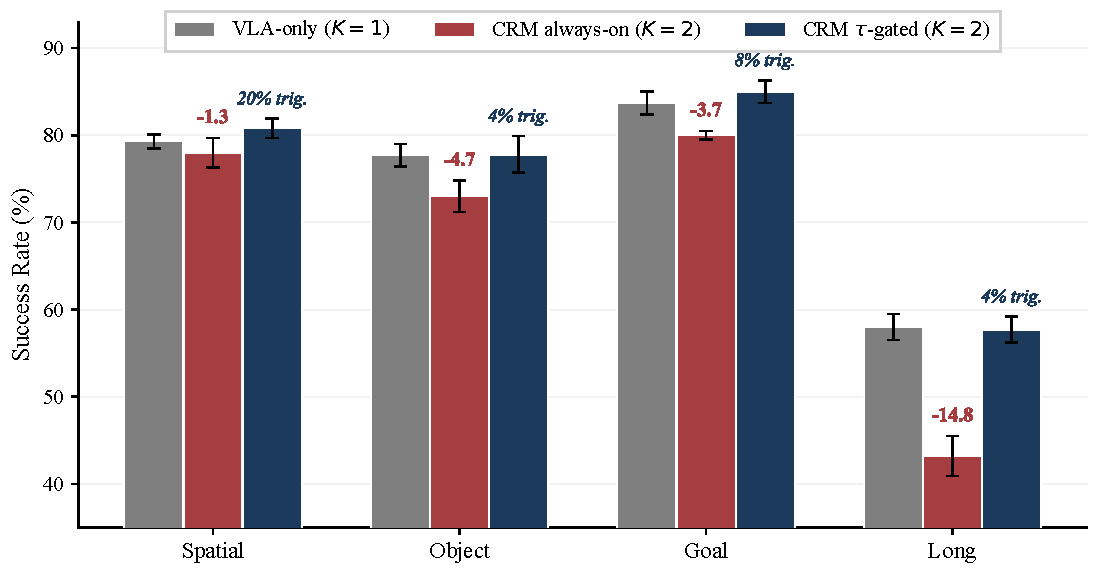
\includegraphics[width=0.8\linewidth]{fig_method_bar.pdf}
  \caption{Success rates across four LIBERO suites under the K-matched comparison. CRM always-on ($K{=}2$, red) degrades all four suites relative to VLA-only; CRM $\tau$-gated ($K{=}2$, dark blue) recovers nearly all degradation by selectively gating correction via calibrated uncertainty gating. Error bars: $\pm$1 std over $n{=}3$ seeds.}
  \label{fig:method_bar}
\end{figure}

Table~\ref{tab:main} and Figure~\ref{fig:method_bar} report task success rates. Unconditional correction degrades all four suites (Figure~\ref{fig:teaser}): $-$14.8\,pp on Long ($58.0{\to}43.2$\%), $-$4.7\,pp on Object, $-$3.7\,pp on Goal, $-$1.3\,pp on Spatial. The CRM applies a learned residual at every step, including the 80--97\% where the VLA is already confident; on these steps, corrections are noise. Calibrated $\tau$-gating recovers nearly all degradation, yielding $\Delta_{\tau\text{-gated}}$ (vs.\ VLA-only) of $+$1.5\,pp on Spatial (trigger ${\sim}$20\%), $+$1.1\,pp on Goal (trigger ${\sim}$8\%), and baseline-preserving on Object ($+$0.1\,pp, trigger ${\sim}$4\%) and Long ($-$1.3\,pp; $n{=}5$: $-$0.3\,pp$^\dagger$, trigger ${\sim}$4\%). Long, where the CRM is out-of-distribution, provides the clearest signal: unconditional correction loses 14.8\,pp; calibrated gating at ${\sim}$4\% trigger rate recovers 13.5\,pp of that degradation ($\Delta_{\mathrm{gate}}{=}{+}13.5$ vs.\ CRM always-on). An 8-seed analysis on Spatial yields $p{=}0.017$ (Appendix~\ref{sec:8seed}). Across all eight suite${\times}$VLA configurations (four SmolVLA $+$ four $\pi_{0.5}$), CRM always-on consistently degrades performance relative to VLA-only (one-sided sign test, $p = (1/2)^{8} {=} 0.004$), establishing that unconditional correction is harmful regardless of task difficulty or model scale. Moreover, 7 of 8 individual per-suite comparisons reach statistical significance at $\alpha{=}0.05$ (two-sample $t$-test, $n{=}3$ per condition); the sole exception is SmolVLA Spatial ($\Delta{=}{-}1.3$\,pp, $p{\approx}0.30$), where the small effect size ($d{=}1.0$) limits power at $n{=}3$. Gating matches or exceeds unconditional correction in 7 of 8 suite${\times}$VLA configurations (one-sided sign test, $p{=}0.035$); the single exception ($\pi_{0.5}$ Object, VLA-only 99.3\%) aligns with Rule~5. CRM degradation effect sizes are uniformly large (Cohen's $d{=}1.0$--$7.6$ on SmolVLA, $d{=}2.9$--$13.2$ on $\pi_{0.5}$), confirming that the harmful pattern is not a marginal effect.

\subsection{Correlation Between Trigger Rate and Net Improvement}
\label{sec:trigger_correlation}

\begin{wrapfigure}{r}{0.44\textwidth}
  \centering
  \vspace{-12pt}
  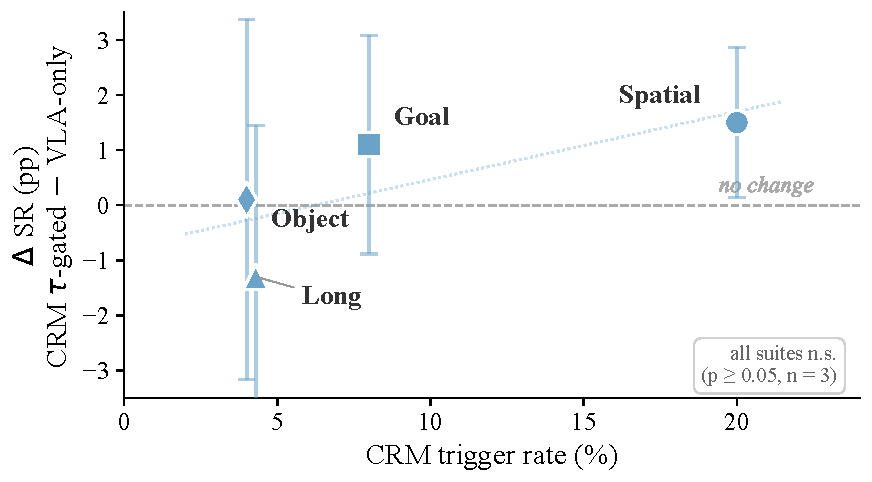
\includegraphics[width=0.42\textwidth]{fig_trigger_scatter.pdf}
  \caption{Trigger rate vs.\ improvement over VLA-only ($\Delta_{\tau\text{-gated}}$). Higher trigger $\to$ larger gain; low-trigger suites preserve baseline.}
  \label{fig:trigger_scatter}
  \vspace{-8pt}
\end{wrapfigure}

\begin{table}[t]
\centering
\caption{Cross-VLA validation on $\pi_{0.5}$ (3.6B). Unconditional CRM correction degrades all four suites, with Long suffering $-$17.5\,pp---the largest degradation across both VLAs. $n{=}3$ seeds per condition; full results including gating in Appendix Table~\ref{tab:pi05_multiseed}.}
\label{tab:pi05_main}
\small
\begin{tabular}{lccc}
\toprule
Suite & VLA-only & CRM always-on & $\Delta_{\mathrm{CRM}}$ \\
\midrule
Spatial & $98.0 \pm 0.5$ & $96.8 \pm 0.3$ & $-1.2$ \\
Object & $99.3 \pm 0.8$ & $88.0 \pm 1.0$ & $-11.3$ \\
Goal & $97.5 \pm 0.5$ & $84.5 \pm 1.3$ & $-13.0$ \\
Long & $95.0 \pm 0.9$ & $77.5 \pm 1.8$ & $\mathbf{-17.5}$ \\
\bottomrule
\end{tabular}
\end{table}

Figure~\ref{fig:trigger_scatter} visualizes the mechanism: trigger rate shows a positive trend with net improvement over VLA-only ($\Delta_{\tau\text{-gated}}$) across the four evaluated suites. Suites with high uncertainty (trigger ${>}$7\%: Spatial, Goal) see positive corrections; confident suites (trigger ${<}$5\%: Object, Long) preserve baseline, avoiding the catastrophic $-$14.8\,pp and $-$4.7\,pp degradation of unconditional correction. $\tau$-sweep analysis (Appendix Figure~\ref{fig:tau_sweep}a) shows SR varies by ${\leq}$2\,pp over a $3{\times}$ range of $\tau$, confirming that practitioners need not precisely tune the threshold. CRM corrections are robust across all magnitudes $\varepsilon \leq 0.2$ when conditioned on observation features (Appendix Figure~\ref{fig:tau_sweep}b). Notably, trigger rates are highly stable across seeds (SD ${\leq}$0.9\,pp across all suites), indicating that trigger rate is a suite-level characteristic rather than a stochastic artifact---a single validation run suffices for deployment diagnostics. This monotonic relationship makes trigger rate a zero-cost deployment diagnostic: evaluating it on a small validation set suffices to predict whether correction will yield positive gains or merely preserve baseline.

The suite-level pattern reflects task-specific uncertainty structure. Spatial tasks require precise placement relative to landmarks, producing genuinely diverse candidates when the VLA hesitates; the CRM resolves this ambiguity productively. Goal tasks involve varied goal specifications that occasionally produce uncertain predictions, yielding moderate trigger rates (${\sim}$8\%) and consistent $+$1.1\,pp gains. Object tasks involve novel instances where pretrained representations generalize well, yielding confident predictions that correction can only perturb. Long, where the CRM is out-of-distribution, confirms that gating effectiveness depends jointly on VLA uncertainty quality and CRM coverage; here the gate's conservative ${\sim}$4\% trigger rate prevents the CRM from injecting out-of-distribution noise on 96\% of steps, recovering 13.5 of the 14.8\,pp degradation.

\paragraph{Efficiency.}
Under batched inference with shared prefix encoding, $K{=}2$ latency matches $K{=}1$ (${\sim}$170\,ms), making the uncertainty probe computationally free. CRM adds ${\sim}$0.25\,ms per call; $\tau$-gating invokes it on only 4--20\% of steps (Table~\ref{tab:efficiency}).

\begin{table}[t]
\centering
\caption{Computational comparison. CRM $\tau$-gated and CRM always-on share the same $K{=}2$ VLA cost; the difference is CRM invocation frequency. CRM overhead per call is negligible (${\sim}$0.25\,ms).}
\label{tab:efficiency}
\small
\begin{tabular}{lccc}
\toprule
Method & VLA calls & Latency (ms) & CRM calls (\%) \\
\midrule
VLA-only & 1 & ${\sim}$170 & 0 \\
CRM always-on & 2 & ${\sim}$170 & 100 \\
\textbf{CRM $\tau$-gated} & \textbf{2} & $\mathbf{{\sim}170}$ & \textbf{4--20} \\
\bottomrule
\end{tabular}
\end{table}

Cross-VLA validation on $\pi_{0.5}$~\cite{black2025pi05} (3.6B) confirms with $n{=}3$ per condition that the degradation pattern persists and amplifies across model scale (Table~\ref{tab:pi05_main}): unconditional CRM correction degrades all four suites, with $-$17.5\,pp on Long---the largest degradation across both VLAs. Full results including gating are in Appendix Table~\ref{tab:pi05_multiseed}. The degradation is larger on $\pi_{0.5}$ than SmolVLA on three of four suites, suggesting that stronger base models produce more confident actions that are even more sensitive to noise injection from unconditional correction. A boundary analysis on OpenVLA-OFT~\cite{kim2024openvla} (7B, deterministic) shows that stochastic diversity is a prerequisite for multi-sample calibrated scoring: deterministic VLAs produce near-identical samples across forward passes, yielding $d_2 \approx 0$ and rendering the pairwise distance probe uninformative (Appendix~\ref{sec:applicability}). This establishes an explicit applicability boundary: the pipeline requires flow-matching or diffusion-based VLAs that produce genuinely diverse samples.

\paragraph{Deployment Guidelines.}
\looseness=-1 Our cross-suite and cross-VLA analysis yields five actionable rules:
\textit{(1)~Require stochastic VLAs.} Deterministic models produce near-identical $K{=}2$ samples, yielding $d_2 \approx 0$ (Appendix~\ref{sec:applicability}).
\textit{(2)~Train the CRM on deployment tasks.} Leave-task-out SR drops from ${\sim}$78\% to ${\sim}$2\% (Appendix~\ref{sec:reproducibility}); the CRM must cover the target task distribution.
\textit{(3)~Use trigger rate as a diagnostic.} Trigger rate ${>}$7\% predicts positive correction (Spatial $+$1.5\,pp at ${\sim}$20\%; Table~\ref{tab:main}); below ${<}$5\%, correction adds little (Object $+$0.1\,pp at ${\sim}$4\%).
\textit{(4)~$\tau$ selection is forgiving.} SR varies by ${\leq}$2\,pp over a $3{\times}$ range of $\tau$ (Table~\ref{tab:tau_sweep}); choosing a suboptimal threshold has low cost.
\textit{(5)~Do not correct near-expert VLAs.} When baseline SR exceeds ${\sim}$95\%, both unconditional and gated correction degrade performance ($\pi_{0.5}$; Tables~\ref{tab:pi05_main},~\ref{tab:pi05_multiseed}).



\section{Conclusion}
\label{sec:conclusion}

\looseness=-1 We showed that learned post-hoc correction of frozen flow-matching VLAs is harmful by default. Under a K-matched comparison, unconditional correction degrades all four LIBERO suites on SmolVLA (0.4B) and all four on $\pi_{0.5}$ (3.6B), with the largest degradation on Long where the CRM is out-of-distribution. The root cause is that the vast majority of steps are already confident; corrections on these steps inject noise. Calibrated gating via $K{=}2$ pairwise $L_2$ distances detects confident steps and gates the CRM, recovering nearly all degradation on SmolVLA. The trigger rate shows a positive trend with improvement across suites, providing a built-in diagnostic. Because $K{=}2$ batched inference matches $K{=}1$ latency, the uncertainty probe is computationally free. The key finding is that \emph{knowing when not to correct} matters more than correction strength.
Task-agnostic CRM architectures that generalize beyond training tasks would remove the per-task retraining bottleneck; combining temporal correction~\cite{a2c2_2025} with our initial-action gating could address complementary failure modes; and real-robot validation under distribution shift would establish practical deployment viability.

\paragraph{Limitations.}
\label{sec:limitations}
\looseness=-1 The finding applies to the tested MLP-based CRM (${\sim}$327K parameters); larger correction architectures (e.g., transformer-based residual modules) may exhibit different failure modes. The $K{=}2$ probe requires diverse stochastic samples; deterministic VLAs such as OpenVLA-OFT produce near-identical outputs, yielding no usable uncertainty signal (Appendix~\ref{sec:applicability}), restricting applicability to flow-matching or diffusion-based policies. The threshold $\tau$ is a per-suite fixed value tuned on validation rollouts rather than learned end-to-end; an adaptive $\tau$ selection mechanism could improve robustness across task distributions. The CRM does not generalize to unseen tasks (leave-task-out SR ${\sim}$2\%), requiring practitioners to collect task-specific rollout data before applying correction, which limits plug-and-play deployment. Recovery on $\pi_{0.5}$ is partial (Table~\ref{tab:pi05_multiseed}), and all experiments use LIBERO simulation; real-robot transfer under visual and dynamics distribution shift remains future work. More broadly, the current CRM architecture does not surpass the VLA-only baseline---adaptive gating recovers the degradation introduced by unconditional correction but does not yield net performance gains beyond noise on SmolVLA, and only partial recovery on $\pi_{0.5}$. The primary contribution is therefore diagnostic and methodological (identifying when correction is harmful and providing a safe deployment framework) rather than achieving absolute performance improvement. Future work on task-agnostic correction architectures may close this gap.


\bibliography{references}

\clearpage

\appendix

\section{Applicability Boundary: Stochastic VLA Diversity}
\label{sec:applicability}

\looseness=-1 The multi-sample pipeline requires stochastic action diversity across samples. We validate this prerequisite on two VLA architectures: SmolVLA~\cite{shukor2025smolvla} (flow matching, 0.4B) and OpenVLA-OFT~\cite{kim2024openvla} (deterministic $L_1$ regression, 7B).

SmolVLA produces meaningfully diverse action samples across all dimensions via its flow-matching generative process. In contrast, OpenVLA-OFT's deterministic $L_1$ regression produces near-identical outputs: mean pairwise $L_2{=}0.00436$ across $K{=}2$ samples, with $97.3$\% of steps below $0.01$. The uncertainty gate never fires, and multi-sample selection is vacuous.

This result establishes an architectural boundary: multi-sample inference-time correction is specific to stochastic generative VLAs (flow matching, diffusion). Deterministic VLAs lack the action diversity that selection and correction rely on. The boundary is architectural, not a limitation of our method: any inference-time approach that draws multiple action candidates requires the base policy to produce diverse samples.

\section{Cross-VLA Analysis: Model Capability Dependency}
\label{sec:cross_vla}

\looseness=-1 We evaluate the CRM degradation pattern on $\pi_{0.5}$~\cite{black2025pi05} (3.6B, flow matching), where near-saturated baselines reach 94--98\% (Table~\ref{tab:pi05}). The same K-matched design ($K{=}2$, $\varepsilon{=}0.2$, shared CRM architecture) is used. Unconditional CRM correction degrades all four suites: Long suffers $-$17.0\,pp ($94.0{\to}77.0$\%, the largest single-suite drop across both VLAs), Goal $-$14.0\,pp, Object $-$6.0\,pp, and Spatial $-$2.0\,pp. Multi-seed evaluation ($n{=}3$; Table~\ref{tab:pi05_multiseed}) confirms the pattern, with Long degradation reaching $-$17.5\,pp. As on SmolVLA, the CRM is trained on three suites and Long is out-of-distribution, amplifying the harm. The degradation on all four suites of both VLAs is consistent with the core thesis: when most steps are already near-optimal, learned correction noise has proportionally greater impact, and this pattern generalizes across model scale.

\begin{table}[h]
\centering
\caption{Cross-VLA degradation analysis: $\pi_{0.5}$ (3.6B) on LIBERO. Near-saturated baselines (94--98\%) are degraded by unconditional CRM correction on all four suites, with Long suffering $-$17.0\,pp (the largest single-seed drop across both VLAs).}
\label{tab:pi05}
\small
\begin{tabular}{lccc}
\toprule
Suite & VLA-only ($K{=}1$) & CRM always-on ($K{=}2$) & $\Delta_{\mathrm{CRM}}$ \\
\midrule
Spatial & $98.0$ & $96.0$ & $-2.0$ \\
Object & $96.5$ & $90.5$ & $-6.0$ \\
Goal & $95.5$ & $81.5$ & $-14.0$ \\
Long & $94.0$ & $77.0$ & $-17.0$ \\
\bottomrule
\addlinespace[2pt]
\multicolumn{4}{l}{\scriptsize $n{=}1$ seed; $\varepsilon{=}0.2$, same CRM architecture as SmolVLA.}\\
\multicolumn{4}{l}{\scriptsize VLA-only and CRM always-on evaluated on different servers (seed-matched); cross-server}\\
\multicolumn{4}{l}{\scriptsize variance is ${\leq}$4\,pp on short suites, and all degradation directions are consistent.}
\end{tabular}
\end{table}


\section{Threshold Sensitivity Analysis}
\label{sec:tau_sweep}

\begin{figure}[h]
  \centering
  \begin{minipage}[t]{0.48\linewidth}
    \centering
    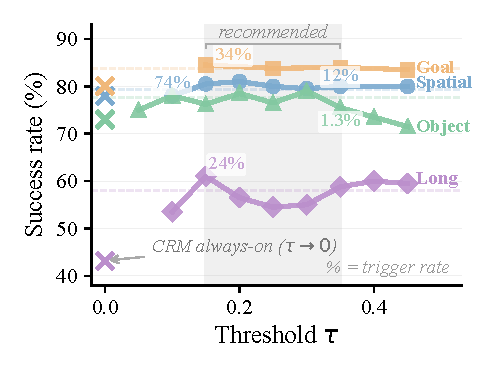
\includegraphics[width=\linewidth]{fig_tau_sweep.pdf}\\[-2pt]
    {\small (a)}
  \end{minipage}
  \hfill
  \begin{minipage}[t]{0.48\linewidth}
    \centering
    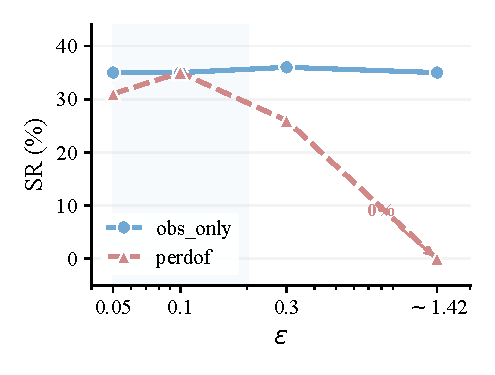
\includegraphics[width=\linewidth]{magnitude_curve.pdf}\\[-2pt]
    {\small (b)}
  \end{minipage}
  \caption{(a)~Threshold sensitivity on SmolVLA. Solid: CRM $\tau$-gated SR; dashed: VLA-only baselines; $\times$: CRM always-on. SR varies by ${\leq}$2\,pp over a $3{\times}$ range of $\tau$. (b)~Correction magnitude sensitivity on Spatial (seed 42): observation-only CRM (blue) is robust across $\varepsilon \in [0.05, 0.2]$; per-DOF variant (red) collapses at high $\varepsilon$.}
  \label{fig:tau_sweep}
\end{figure}

\begin{table}[h]
\centering
\caption{SmolVLA threshold sensitivity ($\varepsilon{=}0.2$), complete $\tau$-sweep across all four LIBERO suites. $\tau$ primarily controls intervention frequency: on Spatial ($\tau{=}0.15$--$0.45$), trigger rate changes $5.5{\times}$ while SR varies by ${\leq}$2\,pp. Long is out-of-distribution (OOD) for the CRM (Section~\ref{sec:exp_setup}).}
\label{tab:tau_sweep}
\small
\begin{tabular}{llccc}
\toprule
Suite & $\tau$ & SR (\%) & Trigger (\%) & $n$ \\
\midrule
Spatial & 0.10 & 78.0 & 74.4 & 1 \\
Spatial & 0.15 & 80.5 & 40.7 & 1 \\
Spatial & 0.20 & 81.0 & 26.7 & 1 \\
Spatial & 0.25 & 80.0 & 19.5 & 3 \\
Spatial & 0.30 & 79.5 & 16.8 & 1 \\
Spatial & 0.35 & 80.0 & 12.2 & 1 \\
Spatial & 0.45 & 80.0 & 7.3 & 1 \\
\midrule
Goal & 0.15 & 84.5 & 34.4 & 2 \\
Goal & 0.25 & 83.8 & 8.1 & 3 \\
Goal & 0.35 & 84.0 & 2.3 & 2 \\
Goal & 0.45 & 83.5 & 0.9 & 1 \\
\midrule
Object & 0.05 & 75.0 & --- & 1 \\
Object & 0.10 & 78.0 & --- & 1 \\
Object & 0.15 & 76.2 & 16.6 & 3 \\
Object & 0.20 & 78.5 & --- & 1 \\
Object & 0.25 & 76.5 & 3.5 & 2 \\
Object & 0.30 & 79.0 & 2.3 & 1 \\
Object & 0.35 & 75.5 & 1.3 & 1 \\
Object & 0.40 & 73.5 & 0.9 & 1 \\
Object & 0.45 & 71.5 & 0.8 & 1 \\
\midrule
Long$^{\dagger}$ & 0.10 & 53.5 & 61.3 & 1 \\
Long$^{\dagger}$ & 0.15 & 61.0 & 23.8 & 2 \\
Long$^{\dagger}$ & 0.20 & 56.5 & 8.9 & 2 \\
Long$^{\dagger}$ & 0.25 & 54.5 & 4.4 & 2 \\
Long$^{\dagger}$ & 0.30 & 55.0 & --- & 2 \\
Long$^{\dagger}$ & 0.35 & 58.8 & 1.2 & 2 \\
Long$^{\dagger}$ & 0.40 & 60.0 & 0.4 & 1 \\
Long$^{\dagger}$ & 0.45 & 59.5 & 0.3 & 1 \\
\bottomrule
\addlinespace[2pt]
\multicolumn{5}{l}{\scriptsize $n$: seeds averaged. ${}^{\dagger}$CRM is OOD on Long (trained on 3 suites).}\\
\multicolumn{5}{l}{\scriptsize ---: trigger rate not recorded for this run.}
\end{tabular}
\end{table}

\begin{table}[h]
\centering
\caption{$\pi_{0.5}$ threshold sensitivity ($\varepsilon{=}0.2$). The plateau pattern holds on the three evaluated suites (Spatial, Goal, Long): trigger rate varies substantially with $\tau$, but SR changes remain small. Extended $\tau$ range on Goal ($0.15$--$0.90$) suggests robustness.}
\label{tab:tau_sweep_pi05}
\small
\begin{tabular}{llccc}
\toprule
Suite & $\tau$ & SR (\%) & Trigger (\%) & $n$ \\
\midrule
Spatial & 0.15 & 97.0 & 11.2 & 1 \\
Spatial & 0.25 & 96.8 & 4.4 & 2 \\
Spatial & 0.35 & 96.5 & 2.6 & 1 \\
\midrule
Goal & 0.15 & 92.0 & 17.4 & 1 \\
Goal & 0.25 & 87.5 & 9.1 & 3 \\
Goal & 0.35 & 87.5 & 5.7 & 1 \\
Goal & 0.50 & 87.0 & 2.1 & 1 \\
Goal & 0.70 & 87.0 & 1.0 & 1 \\
Goal & 0.90 & 89.0 & 0.4 & 1 \\
\midrule
Long & 0.15 & 84.0 & 11.4 & 1 \\
Long & 0.25 & 81.0 & 4.4 & 3 \\
Long & 0.35 & 81.0 & 2.4 & 1 \\
\bottomrule
\end{tabular}
\end{table}

\looseness=-1 Tables~\ref{tab:tau_sweep} and~\ref{tab:tau_sweep_pi05} report success rates as a function of the uncertainty threshold $\tau$ on SmolVLA and $\pi_{0.5}$, respectively. On both models, $\tau$ primarily controls intervention frequency rather than final SR: on SmolVLA Spatial, trigger rate drops from 40.7\% ($\tau{=}0.15$) to 7.3\% ($\tau{=}0.45$), a $5.5{\times}$ reduction, while SR varies by only 1.5\,pp (79.5--81.0\%). On $\pi_{0.5}$ Spatial, a similar pattern holds (11.2\%$\to$2.6\% trigger, 0.5\,pp SR range). This plateau effect indicates that the CRM needs to intervene on only a small fraction of steps to reach its performance ceiling.

\looseness=-1 The Long suite, where the CRM is OOD, exhibits wider SR variation across $\tau$: from 53.5\% ($\tau{=}0.10$, trigger 61.3\%) to 61.0\% ($\tau{=}0.15$, trigger 23.8\%). Notably, $\tau{=}0.15$ exceeds VLA-only (58.0\%) by 3\,pp, while the shared threshold $\tau{=}0.25$ yields 54.5\%. This suite-dependence of optimal $\tau$ motivates adaptive threshold selection as future work (Section~\ref{sec:limitations}). On $\pi_{0.5}$ Goal, extending $\tau$ from 0.15 to 0.90 confirms the plateau: SR remains within 87.0--92.0\% as trigger rate drops from 17.4\% to 0.4\%.

\looseness=-1 Goal shows a stable plateau (${\sim}$1\,pp variation, 83.5--84.5\%) across $\tau$, within per-seed noise (Table~\ref{tab:main}, std ${\sim}$1--2\,pp). Object exhibits wider variation: SR ranges from 71.5\% ($\tau{=}0.45$) to 79.0\% ($\tau{=}0.30$), a 7.5\,pp spread. At high $\tau$ (${\geq}0.35$), Object SR degrades because the gate rarely fires (${\leq}$1.3\%) and $K{=}2$ argmin alone underperforms VLA-only on this suite. The within-suite relationship between trigger rate and SR is not monotonic, consistent with the CRM providing limited correction quality on steps where the VLA's errors are systematic rather than stochastic. The cross-suite positive correlation (higher trigger rate correlating with larger improvement, Figure~\ref{fig:trigger_scatter}) remains the primary mechanism evidence.

\looseness=-1 \textbf{Note on $\varepsilon$.}\enspace Both CRM always-on and CRM $\tau$-gated in Table~\ref{tab:main} use $\varepsilon{=}0.2$, matching the $\tau$-sweep configuration. The K-matched design ensures the only variable is calibrated gating ($\tau{\to}0$ vs.\ calibrated $\tau$).


\section{Uncertainty Proxy Comparison}
\label{sec:proxy_comparison}

\looseness=-1 Table~\ref{tab:proxy_comparison} (main text) compares four candidate uncertainty proxies against $K{=}10$ sample variance as ground truth. CRM correction magnitude (the $L_2$ norm of the CRM's predicted residual) is attractive because it requires no extra VLA forward passes, but correlates weakly with true uncertainty ($\rho < 0.16$): the CRM predicts similar-magnitude corrections regardless of whether the VLA is confident or uncertain. FMVD, which measures dispersion in the flow-matching velocity field, performs worse still ($\rho{=}0.083$). The $K{=}2$ pairwise $L_2$ distance achieves near-perfect correlation ($\rho{=}0.9979$) at the cost of one additional VLA forward pass, which is absorbed by batched inference (Section~\ref{sec:efficiency}).


\section{Reproducibility Details}
\label{sec:reproducibility}

\paragraph{Hardware.}
All experiments run on NVIDIA RTX 4090 GPUs (24\,GB VRAM). SmolVLA inference uses a single GPU; CRM training and evaluation each use a single GPU.

\paragraph{CRM training.}
The CRM is trained on three suites (Spatial, Object, Goal; 30 tasks, ${\sim}$88K samples) for 50 epochs with Adam ($\mathrm{lr}{=}10^{-3}$, batch size 32) in ${\sim}$6 GPU-hours on 1$\times$ RTX 4090. Long is excluded from CRM training; Long-suite evaluation tests cross-suite generalization. Precomputing the $K{=}10$ forward-pass cache (required once per suite) takes ${\sim}$2 GPU-hours per suite.

\paragraph{Evaluation.}
Each suite evaluation (20 rollouts $\times$ 10 tasks $\times$ 300 max steps) takes ${\sim}$2.5 GPU-hours. A full 5-method $\times$ 4-suite $\times$ 3-seed experiment requires ${\sim}$150 GPU-hours total.

\paragraph{Software.}
PyTorch 2.4, Transformers 4.45, LIBERO (MuJoCo-based). Code and CRM checkpoints will be released upon acceptance.


\section{Computational Efficiency}
\label{sec:efficiency}

Table~\ref{tab:efficiency} (main text) compares the computational cost of each method. The key insight is that batched inference absorbs the cost of the second VLA forward pass: $K{=}2$ latency matches $K{=}1$ because both samples share the same prefix encoding and flow-matching denoising runs in parallel.


\section{Extended 8-Seed Analysis on Spatial}
\label{sec:8seed}

\begin{table}[h]
\centering
\caption{Per-seed success rates (\%) on LIBERO-Spatial for VLA-only vs.\ CRM $\tau$-gated ($K{=}2$, $\tau{=}0.25$). All 8 seeds use identical $K{=}2$ configuration (code-verified).}
\label{tab:8seed}
\small
\begin{tabular}{lccc}
\toprule
Seed & VLA-only & CRM $\tau$-gated & $\Delta$ \\
\midrule
42 & 80.0 & 82.0 & $+2.0$ \\
43 & 79.0 & 80.0 & $+1.0$ \\
44 & 78.5 & 80.5 & $+2.0$ \\
45 & 80.0 & 80.0 & $+0.0$ \\
46 & 80.5 & 80.0 & $-0.5$ \\
47 & 80.0 & 81.5 & $+1.5$ \\
48 & 79.5 & 81.0 & $+1.5$ \\
49 & 78.5 & 82.0 & $+3.5$ \\
\midrule
Mean$\pm$std & $79.5 \pm 0.8$ & $80.9 \pm 0.9$ & $+1.4$ \\
\bottomrule
\end{tabular}
\end{table}

\looseness=-1 Table~\ref{tab:8seed} reports per-seed results for the extended 8-seed paired analysis on LIBERO-Spatial. A paired $t$-test yields $\Delta{=}{+}1.4$\,pp, $p{=}0.017$ ($n{=}8$), reaching statistical significance at $\alpha{=}0.05$. Six of eight seeds show positive $\Delta$; the two non-positive seeds ($\Delta{=}0.0$ and $\Delta{=}{-}0.5$) are consistent with measurement noise rather than systematic degradation. This analysis provides the strongest statistical evidence that calibrated $\tau$-gating produces a genuine improvement on the suite where the uncertainty gate fires most frequently (trigger rate ${\sim}$20\%).


\section{Additional Ablations}
\label{sec:additional_ablations}

\begin{table}[h]
\centering
\caption{Supplementary ablations on SmolVLA. $K{=}10$ argmin~\cite{chen2026reconvla}: argmin-to-centroid selection over 10 samples, no learned correction. $K{=}2$ mean: centroid of two samples, no CRM. Neither consistently improves over VLA-only.}
\label{tab:ablations}
\small
\begin{tabular}{lcccccc}
\toprule
Method & $K$ & Spatial (\%) & Object (\%) & Goal (\%) & Long (\%) \\
\midrule
VLA-only & 1 & $79.3 \pm 0.8$ & $77.7 \pm 1.3$ & $83.7 \pm 1.3$ & $58.0 \pm 1.5$ \\
$K{=}10$ argmin & 10 & $80.3 \pm 1.0$ & $77.3 \pm 1.5$ & $80.8 \pm 0.3$ & $56.5^{\dagger}$ \\
$K{=}2$ mean & 2 & --- & $77.5 \pm 2.3$ & $83.0 \pm 2.2$ & $57.0^{\dagger}$ \\
\bottomrule
\addlinespace[2pt]
\multicolumn{6}{l}{\scriptsize $n{=}3$ seeds unless noted; ${}^{\dagger}n{=}1$; --- = omitted (computational budget).}
\end{tabular}
\end{table}

\looseness=-1 Table~\ref{tab:ablations} reports two ablations that isolate multi-sample selection without learned correction. $K{=}10$ argmin invests $10{\times}$ the VLA forward passes but hurts on Goal ($-$2.9\,pp) and Long ($-$1.5\,pp): selection alone cannot fix systematic errors. $K{=}2$ mean offers no learned correction mechanism ($-$0.7\,pp Goal, $-$1.0\,pp Long; Long is single-seed preliminary), confirming that multi-sampling alone is insufficient.


\section{CRM Always-On Per-Seed Analysis}
\label{sec:crm_perseed}

\begin{table}[h]
\centering
\caption{Per-seed success rates (\%) for CRM always-on ($K{=}2$, $\varepsilon{=}0.2$, $\tau{\to}0$). SmolVLA uses seeds 42--46 ($n{=}5$); Table~\ref{tab:main} reports $n{=}3$ means from seeds 42--44. $\pi_{0.5}$ rows show fewer seeds; full multi-seed results in Table~\ref{tab:pi05_multiseed}.}
\label{tab:crm_perseed}
\small
\begin{tabular}{llccccccc}
\toprule
Model & Suite & s42 & s43 & s44 & s45 & s46 & $n$ & Mean$\pm$Std \\
\midrule
SmolVLA & Spatial & 79.0 & 76.0 & 79.0 & 77.0 & 78.5 & 5 & $77.9 \pm 1.3$ \\
SmolVLA & Object & 71.0 & 73.5 & 74.5 & 74.5 & 67.5 & 5 & $72.2 \pm 3.0$ \\
SmolVLA & Goal & 80.0 & 79.5 & 80.5 & 82.0 & 80.0 & 5 & $80.4 \pm 1.0$ \\
SmolVLA & Long & 41.0 & 45.5 & 43.0 & --- & --- & 3 & $43.2 \pm 2.3$ \\
\midrule
$\pi_{0.5}$ & Spatial & 96.0 & --- & --- & --- & --- & 1 & $96.0$ \\
$\pi_{0.5}$ & Object & 90.5 & 92.0 & --- & --- & --- & 2 & $91.2 \pm 1.1$ \\
$\pi_{0.5}$ & Goal & 81.5 & --- & --- & --- & --- & 1 & $81.5$ \\
$\pi_{0.5}$ & Long & 77.0 & --- & --- & --- & --- & 1 & $77.0$ \\
\bottomrule
\addlinespace[2pt]
\multicolumn{9}{l}{\scriptsize ---: not evaluated. SmolVLA Long s45 incomplete (excluded).}
\end{tabular}
\end{table}

\looseness=-1 Table~\ref{tab:crm_perseed} reports per-seed CRM always-on results. SmolVLA means over seeds 42--44 match Table~\ref{tab:main}; the extended 5-seed means show consistent degradation patterns across all suites. Object exhibits the highest per-seed variance (std${=}$3.0), driven by seed 46 (67.5\%), suggesting interaction between CRM noise injection and task-specific stochasticity.


\section{\texorpdfstring{$\pi_{0.5}$}{Pi-0.5} Extended Multi-Seed Results}
\label{sec:pi05_multiseed}

\begin{table}[h]
\centering
\caption{$\pi_{0.5}$ (3.6B) per-seed success rates (\%) across three methods and four LIBERO suites from dedicated multi-seed evaluation runs. Table~\ref{tab:pi05} reports seed-42 matched pairs from separate runs; per-seed differences (${\leq}$4\,pp) reflect cross-server variance and evaluation stochasticity.}
\label{tab:pi05_multiseed}
\small
\begin{tabular}{llccccc}
\toprule
Suite & Method & s42 & s43 & s44 & $n$ & Mean$\pm$Std \\
\midrule
Spatial & VLA-only & 98.0 & 97.5 & 98.5 & 3 & $98.0 \pm 0.5$ \\
Spatial & CRM always-on & 96.5 & 97.0 & 97.0 & 3 & $96.8 \pm 0.3$ \\
Spatial & CRM $\tau$-gated & 96.5 & 98.0 & 97.0 & 3 & $97.2 \pm 0.8$ \\
\midrule
Object & VLA-only & 100.0 & 98.5 & 99.5 & 3 & $99.3 \pm 0.8$ \\
Object & CRM always-on & 89.0 & 87.0 & 88.0 & 3 & $88.0 \pm 1.0$ \\
Object & CRM $\tau$-gated & 85.5 & 85.0 & 88.0 & 3 & $86.2 \pm 1.6$ \\
\midrule
Goal & VLA-only & 98.0 & 97.0 & 97.5 & 3 & $97.5 \pm 0.5$ \\
Goal & CRM always-on & 85.5 & 83.0 & 85.0 & 3 & $84.5 \pm 1.3$ \\
Goal & CRM $\tau$-gated & 89.5 & 89.5 & 86.5 & 3 & $88.5 \pm 1.7$ \\
\midrule
Long & VLA-only & 94.0 & 95.5 & 95.5 & 3 & $95.0 \pm 0.9$ \\
Long & CRM always-on & 77.0 & 79.5 & 76.0 & 3 & $77.5 \pm 1.8$ \\
Long & CRM $\tau$-gated & 80.5 & 80.5 & 83.0 & 3 & $81.3 \pm 1.4$ \\
\bottomrule
\addlinespace[2pt]
\multicolumn{7}{l}{\scriptsize VLA-only and CRM evaluated on different servers (seed-matched).}
\end{tabular}
\end{table}

\looseness=-1 Table~\ref{tab:pi05_multiseed} extends the single-seed results in Table~\ref{tab:pi05} to $n{=}3$ seeds per condition on $\pi_{0.5}$. Unconditional CRM correction degrades all four suites relative to VLA-only, confirming the single-seed pattern with $n{=}3$: Long suffers $-$17.5\,pp ($95.0{\to}77.5$), the largest single-suite degradation across both VLAs. On Object, CRM $\tau$-gated ($86.2$\%) performs below CRM always-on ($88.0$\%), indicating that gating recovery depends on the quality of the underlying CRM---which diminishes when the base policy is near-optimal (VLA-only $99.3$\%). On Long, $\tau$-gating recovers 3.8\,pp relative to CRM always-on ($81.3$ vs.\ $77.5$), consistent with OOD suppression. Goal $\tau$-gating ($88.5{\pm}1.7$) partially recovers the $-$13.0\,pp CRM degradation ($97.5{\to}84.5$).


\section{K-Sweep Analysis}
\label{sec:k_sweep}

\begin{table}[h]
\centering
\caption{Effect of sample count $K$ on CRM always-on performance (SmolVLA, LIBERO-Object, $\varepsilon{=}0.2$). Increasing $K$ beyond 2 provides marginal improvement; $K{=}10$ yields the highest SR but at $5{\times}$ the VLA cost.}
\label{tab:k_sweep}
\small
\begin{tabular}{lcccc}
\toprule
$K$ & VLA calls & Seeds & SR (Mean$\pm$Std) & $\Delta$ vs.\ $K{=}2$ \\
\midrule
2 & 2 & 5 & $72.2 \pm 3.0$ & --- \\
5 & 5 & 2 & $73.2 \pm 0.4$ & $+1.0$ \\
10 & 10 & 1 & $78.0$ & $+5.8$ \\
20 & 20 & 2 & $74.5 \pm 1.4$ & $+2.3$ \\
\bottomrule
\addlinespace[2pt]
\multicolumn{5}{l}{\scriptsize $K{=}2$: from Table~\ref{tab:crm_perseed} ($n{=}5$). $K{=}10$ uses $\varepsilon{=}0.05$ (single seed).}
\end{tabular}
\end{table}

\looseness=-1 Table~\ref{tab:k_sweep} varies the sample count $K$ for CRM always-on on LIBERO-Object. Performance is relatively stable across $K{=}2$--$20$ (72.2--78.0\%), with $K{=}10$ showing the highest point estimate but at $5{\times}$ the VLA forward-pass cost and with only a single seed. The marginal gain from larger $K$ does not justify the computational cost, supporting the paper's use of $K{=}2$ with calibrated gating as the preferred operating point.

\section{Negative Results: Alternative CRM Designs}
\label{sec:negative_results}

\looseness=-1 We summarize four design alternatives that were systematically evaluated and failed, providing guidance for future work.

\paragraph{Per-DOF uncertainty conditioning.}
Conditioning the CRM on per-degree-of-freedom uncertainty features (rather than observation-only) causes progressive collapse: with uncapped correction magnitude, SR drops to 0\% consistently across seeds; even at $\varepsilon{=}0.3$, SR recovers only to 4--6\% vs.\ 77\% for observation-only (17 experiments). Exposing per-DOF uncertainty amplifies dimension-correlated correction noise, suggesting that lower-dimensional conditioning is preferable for small CRMs.

\paragraph{Single-sample correction (K=1 CRM with ACCG).}
Bypassing multi-sampling entirely---using a single VLA forward pass with approximate conformal correction guidance (ACCG)---yields SR of 7--12\%, a catastrophic degradation from VLA-only (77.7\%; 8 experiments). Without diverse samples, the pairwise distance gate cannot fire and the CRM receives no useful uncertainty signal. Multi-sampling is a necessary enabler, not merely a convenience.

\paragraph{Leave-task-out generalization.}
When the CRM is evaluated on held-out tasks within the same suite (Object), SR drops to ${\sim}$2\% vs.\ ${\sim}$80\% VLA-only (2 experiments). The CRM is effectively task-set-specific: it memorizes correction patterns for seen tasks rather than learning generalizable residuals. This motivates future work on task-agnostic correction architectures.

\paragraph{Learned uncertainty head.}
Training a separate uncertainty prediction head to replace the $K{=}2$ pairwise distance probe yields SR of 11--14\% with near-zero trigger rates (3 experiments). The effective uncertainty signal arises from the flow-matching process's inherent stochasticity across forward passes, which cannot be captured by a deterministic learned predictor from a single pass.

\smallskip\noindent\textit{AI tools assisted with code and manuscript.}


\end{document}
